\phantomsection

\chapter{Programas em Ipe}\label{chapter:programas-em-ipe}
\phantomsection

Para facilitar o desenvolvimento de aplicações Ipe, todos os programas contam com um conjunto de
bibliotecas padrão, também conhecidas como \textit{Prelude}, que são apresentadas na
\autoref{sec:libpadrao}. Ademais, para manter a pureza dos programas Ipe, a linguagem disponibiliza
um ambiente que faz a gerência de efeitos colaterais, como acesso a disco ou rede. Esse ambiente
é apresentado na \autoref{sec:runtime}.

\section{Bibliotecas padrão}\label{sec:libpadrao}

Ipe oferece módulos para facilitar o uso de seus tipos primitivos (\texttt{Number}
e \texttt{String}), além de módulos para manipulação de listas e dicionários, e
representação de dados opcionais. Essas bibliotecas podem utilizar código Javascript
(a linguagem alvo da compilação) para utilizar otimizações e acessar dados que
não seriam possíveis de acessar em Ipe. O módulo mais importante para o desenvolvimento de
aplicativos backend que respondem a chamadas HTTP é o módulo \texttt{Http} (descrito na
\autoref{sec:lib-http}), que possui funções que são responsáveis por montar a estrutura básica de
uma aplicação web, como a da \autoref{sec:aplicacao-base}.

\subsection{Number}

Este módulo contém algumas funções para manipulação de números, como arrendondamento.
Além disso, como Ipe não possui operadores lógicos (em especial \texttt{==} e \texttt{!=}),
este módulo oferece funções e tipos para comparar números, como mostra o \autoref{lst:number-compare}.

\begin{lstlisting}[label={lst:number-compare},caption={Comparação de números em Ipe}]
type union CompareResult =
    | Smaller
    | Equal
    | Greater

compare : Number -> Number -> CompareResult
\end{lstlisting}

\subsection{String}

O módulo de \texttt{String} contém funções para manipulação de strings, como
concatenação, busca de substrings, e conversão para maiúsculas e minúsculas.

\subsection{Maybe e Result}

Como Ipe não possui nenhum tipo de exceção ou \texttt{null}, os módulos \texttt{Maybe}
e \texttt{Result} são utilizados para representar valores opcionais e resultados
de funções que podem falhar, respectivamente. O \autoref{lst:maybe-result-def}
mostra a definição destes tipos. Este módulo também possui funções para manipular
esses tipos, como as funções \texttt{Maybe.map} e \texttt{Result.map}, que servem
para manipular o conteúdo de um \texttt{Maybe} ou \texttt{Result}, sem precisar
de uma expressão \texttt{match}.

\begin{lstlisting}[label={lst:maybe-result-def},caption={Definição de \texttt{Maybe} e \texttt{Result}}]
type union Maybe content =
    | Nothing
    | Just content

type union Result error ok =
    | Error error
    | Ok ok
\end{lstlisting}


\subsection{List}

O módulo \texttt{List} define funções para lidar com uma das principais estruturas de dado de Ipe.
Internamente, listas são as mesmas listas usadas em Javascript, e podem ser criadas da mesma maneira:
com colchetes. O \autoref{lst:list-def} mostra exemplos de uso de listas, e a implementação da função
\texttt{map}, que modifica o tipo dos elementos de uma lista.

\begin{lstlisting}[label={lst:list-def},caption={Parte do módulo de listas de Ipe}]
split : List element -> Maybe { head : element, tail : List element }
// A implementação de split é feita em Javascript
// split tenta separar o primeiro elemento da lista do resto da lista

insertLeft : element -> List element -> List element
// A implementação de insertLeft é feita em Javascript
// insertLeft adiciona um elemento no início da lista

map : (element -> newElement) -> List element -> List newElement
map =
    \mapFn list ->
        match split list with
            | Nothing -> []
            | Just parts ->
                insertLeft (mapFn parts.head) (map mapFn parts.tail)

empty : List element
empty = []

singleton : element -> List element
singleton =
    \element -> [ element ]

\end{lstlisting}

\subsection{Dict}

Dicionários são coleções de chave-valor dinâmicos. O módulo \texttt{Dict} define
o tipo \texttt{Dict} e funções para manipular dicionários. Por questões de performance
e simplicidade, dicionários são implementados em Javascript.

\subsection{Subscription}

O tipo \texttt{Subscription} é usado pelo ambiente de execução (discutido na
\autoref{sec:runtime}) para sinalizar eventos que ocorrem no sistema e o programa
pode escolher ser notificado para tomar alguma ação.


\subsection{Promise}

\textit{Promises} (ou promessas) são funções que solicitam ações (tarefas) no mundo exterior para
o ambiente de execução, e usam as \textit{Promises} nativas do Javascript. Esse módulo disponibiliza
funções para manipular tarefas, como usar o resultado de uma como entrada de outra. O \autoref{lst:promise-example}
mostra um exemplo de sequenciamento de tarefas.

\begin{lstlisting}[label={lst:promise-example},caption={Exemplo de sequenciamento de tarefas}]
uploadFile : String -> String -> Promise String
uploadFile =
    \fileId destinationUrl ->
        Db.getFilePathById fileId
        |> Promise.andThen File.read
        |> Promise.andThen (\fileContent -> Http.post destinationUrl { body = fileContent })
\end{lstlisting}

A função acima recebe um identificador de arquivo e uma URL de destino, e lê
o caminho do arquivo no banco de dados, lê o arquivo, e envia o conteúdo para
a URL de destino. A função \texttt{Promise.andThen} é usada para encadear as tarefas,
passando o resultado de uma para a outra. Este código é apenas um exemplo, pois
na realidade, teríamos que lidar com erros (usando o tipo \texttt{Result}), e
não apenas com o caso de sucesso.

Para realizar os efeitos colaterais de uma \texttt{Promise}, usamos a função
\texttt{Promise.perform : (Result error ok -> event) -> Promise error ok -> Effect event},
que converte uma \texttt{Promise} em um \texttt{Effect}, que pode ser enviado ao
\textit{runtime}.

\subsection{JSON}

Ipe tem três módulos relacionados a JSON: \texttt{Json}, \texttt{Json.Encode} e \texttt{Json.Decode}.
O módulo \texttt{JSON} define o tipo \texttt{Json}, que representa um valor JSON. O módulo \texttt{Json.Encode}
define funções para transformar valores de Ipe em valores JSON, e o módulo \texttt{Json.Decode} define
funções para transformar valores JSON em valores de Ipe. O \autoref{lst:json-example} mostra um exemplo
de uso desses módulos.

\begin{lstlisting}[label={lst:json-example},caption={Exemplo de uso dos módulos de JSON}]
type alias User =
    { name : String
    , age : Int
    }

encodeUser : User -> Json.Json
encodeUser =
    \user ->
        Json.Encode.object
           [ { field = "name", value = Json.Encode.string user.name }
           , { field = "age", value = Json.Encode.int user.age }
           ]

userDecoder : Json.Decode.Decoder User
userDecoder =
        Json.Decode.object (\name age -> { name = name, age = age })
        |> Json.Decode.field "name" Json.Decode.string
        |> Json.Decode.field "age" Json.Decode.int

\end{lstlisting}

\subsection{Http}\label{sec:lib-http}

O módulo \texttt{Http} define funções para tratar requisições HTTP que o servidor recebe. A função
\texttt{Http.createApp} é a principal função deste módulo, e ela é usada para criar um servidor HTTP
capaz de manter um estado (chamado de \textbf{contexto}) entre respostas. Esta função recebe
configurações para o servidor (como a porta em que ele deve escutar), uma função para construir o
contexto inicial, e uma função que recebe o contexto atual e uma requisição HTTP, e retorna uma
resposta HTTP e um novo contexto. Com esta função, também é possível registrar \texttt{Subscription}s.
O \autoref{chapter:resultados-obtidos} mostra exemplos de uso deste módulo.

\section{Runtime e arquitetura}\label{sec:runtime}

Programas Ipe são desenvolvidos seguindo uma certa arquitetura, também inspirada
pela arquitetura Elm. Programas Ipe são representados por três partes principais:

\begin{itemize}
    \item \textit{Model}: representa o estado do programa. É um tipo definido
          pelo programador -- tipicamente um \texttt{Record}. Também é necessário definir
          uma função \texttt{init} que define o estado inicial do programa. Também
          é possível realizar \textit{Effects} na função de \texttt{init}.
    \item \textit{update}: função que recebe um evento e o estado atual do programa
          (\texttt{Model}). Eventos também são representados por um tipo definido pelo
          programador, e tipicamente são uniões de tipos. A função \texttt{update} possui
          a anotação \texttt{update : event -> model -> \{ model : model, effect : Effect event \}},
          ou seja, recebe um evento e o estado atual do programa, e retorna o novo estado,
          com possíveis efeitos colaterais.
    \item \textit{subscribe}: função que possibilita o programa a se inscrever
          em eventos do sistema, como o recebimento de requisições HTTP. Para tal,
          a função recebe como argumento o \texttt{Model} atual, e retorna uma
          \texttt{Subscription}.
\end{itemize}

O \textit{Runtime} (ambiente de execução, em português) é o responsável por manter
o estado do programa, e executar as funções \texttt{update} e \texttt{subscribe},
além de executar os efeitos colaterais retornados pela função de \texttt{update}.
O \textit{Runtime} é implementado em Javascript, e ele converte \texttt{Promises} em
código Javascript, e retorna o resultado para o programa Ipe.  Similarmente, quando
um programa Ipe adiciona uma nova \texttt{Subscription}, o \textit{Runtime} é
responsável por gerar Javascript que avise o programa Ipe quando necessário. A
\autoref{fig:runtime} mostra uma visão geral do \textit{Runtime} se comunicando
com outras partes do computador.


\begin{figure}[htb]
    \caption{Arquitetura do \textit{Runtime} Ipe}
    \label{fig:runtime}
    \begin{center}
        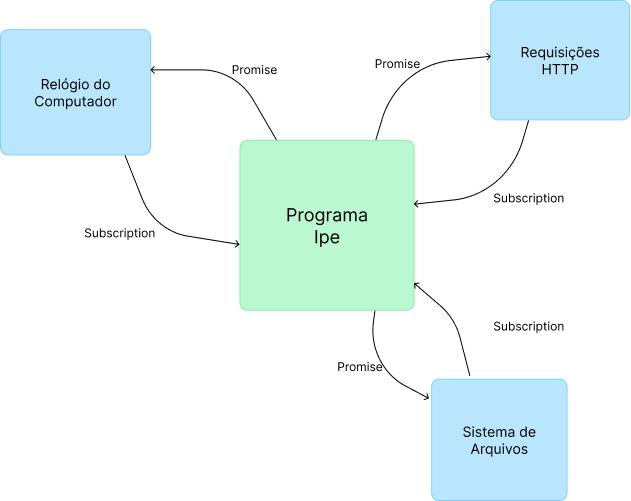
\includegraphics[scale=0.65]{pictures/runtime.png}
    \end{center}
\end{figure}

Para dizer ao \textit{Runtime} quais funções utilizar como funções de inicialização,
\textit{update} e \textit{subscribe}, programas Ipe devem exportar uma função \texttt{main} do módulo
apontado como módulo de entrada (geralmente \texttt{Root.ipe}). O \autoref{lst:full-program} mostra
um exemplo de programa completo em Ipe, que imprime na tela uma mensagem a cada minuto, parando depois
de imprimir 10 vezes.

\begin{lstlisting}[label={lst:full-program},caption={Exemplo de programa completo em Ipe, que imprime na tela uma mensagem a cada minuto}]
module Root exports [main]

type alias Model = { messagesPrinted : Number }

type union Event = 
    | PrintMessage
    | PrintedMessage (Result Console.Error String)

main : { init : { model : Model, effect : Effect Event }
       , update : Event -> Model -> { model : Model, effect : Effect Event }
       , subscribe : Model -> Subscription Event
       }
main =
    { init = { model = { messagesPrinted = 0 }, effect = Effect.none }
    , update = update
    , subscribe = subscribe
    }

update : Event -> Model -> { model : Model, effect : Effect Event }
update =
    \event model ->
        match event with
            | PrintMessage ->
                { model = model
                , effect = 
                    String.fromInt model.messagesPrinted
                    |> Console.log
                    |> Promise.perform PrintedMessage
                }
            | PrintedMessage ->
                { model =
                    { messagesPrinted = model.messagesPrinted + 1 }
                , effect = Effect.none
                }

subscribe : Model -> Subscription Event
subscribe =
    \model ->
        match Number.compare model.messagesPrinted 10 with
            | Number.Smaller -> Time.every 60000 PrintMessage
            | Number.Equal -> Subscription.none
            | Number.Greater -> Subscription.none
\end{lstlisting}

Os passos que o \textit{Runtime} toma para executar o \autoref{lst:full-program}
são:

\begin{enumerate}
    \item Ler a função \texttt{main} para saber quais são as funções \texttt{init},
          \texttt{update} e \texttt{subscribe}.
    \item Executa a função \texttt{init}, e define o estado inicial do programa
          como o \texttt{Record} \texttt{\{ messagesPrinted = 0 \}}. Caso a função \texttt{init}
          retornasse um efeito colateral, o \textit{Runtime} executaria o efeito colateral.
    \item Usa o modelo inicial para executar a função \texttt{subscribe}, e
          começa a esperar por eventos.
    \item Quando um evento chega, o \textit{Runtime} executa a função \texttt{update}
          com o evento e o modelo atual. Efeitos (retornados pelas funções \texttt{init}
          e \texttt{update}) também produzem eventos, que também são tratados na função
          \texttt{update}. Após cada chamada a \texttt{update}, a função \texttt{subscribe}
          é chamada novamente.
    \item Após imprimir 10 vezes na tela, a função \texttt{subscribe} retorna
          \texttt{Subscription.none}, e o programa para de esperar por eventos.
          Quando não existem mais efeitos sendo processados, e a função \texttt{subscribe}
          retorna \texttt{Subscription.none}, o programa termina.
\end{enumerate}

A \autoref{fig:runtime-internals} mostra mais detalhes de como as funções \texttt{init},
\texttt{update} e \texttt{subscribe} se integram com o \textit{Runtime}.

\begin{figure}[htb]
    \caption{Arquitetura detalhada do \textit{Runtime} Ipe}
    \label{fig:runtime-internals}
    \begin{center}
        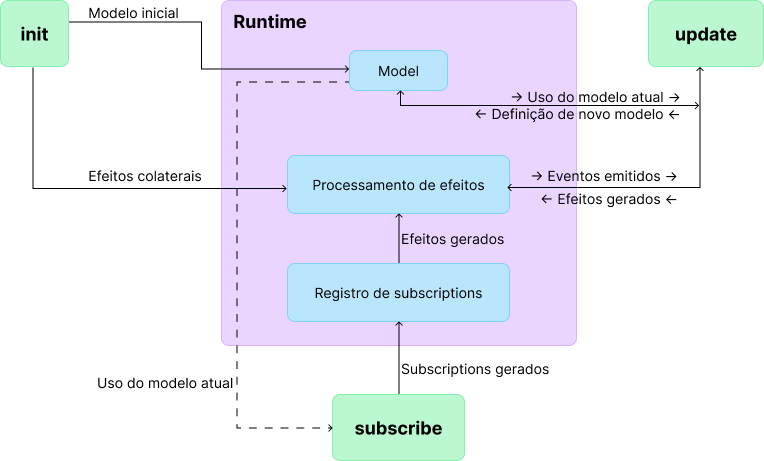
\includegraphics[scale=0.5]{pictures/runtime-internals.png}
    \end{center}
\end{figure}

Podemos ver que, após a definição do modelo inicial em \texttt{init}, as funções
\texttt{update} e \texttt{subscribe} leem o modelo, e respondem a eventos.

Embora este seja o fluxo principal de execução, alguns módulos do \textit{Prelude} de Ipe podem oferecer
funções auxiliares, que ajudam a definir o comportamento do programa, de maneira mais apropriada de
acordo com uma certa necessidade ou contexto. Por exemplo, com \texttt{Http.createApp}, o modelo
passa a se chamar contexto, a função \texttt{init} se chama \texttt{createContext}, e a função
\texttt{update} é substituída pela função \texttt{handleRequest}, de forma que algumas partes do
funcionamento do servidor são omitidas do programador final, como a \texttt{Subscription} que escuta
por requisições HTTP, ou o efeito que envia respostas HTTP.
